\documentclass[a4paper,10pt,oneside,leqno]{scrartcl}
\usepackage[utf8]{inputenc}
\usepackage{listingsutf8}
\usepackage[pdftex]{graphicx}
%\usepackage[ngerman]{babel}
\usepackage{url}
\usepackage{hyperref}
\usepackage{amsfonts}
\usepackage{amssymb}
\usepackage{amsmath}
\usepackage{tikz}
\usepackage{listings}
\usepackage{pdfpages}
\usepackage{textcomp}
\usepackage{amsmath}
%\usepackage{lipsum}%%%%%%%%%%%%%%%%%%%%%%%%%%%%%%%%%%%%%%%%%%%%%%%%%%%%%%%%%%%%%%%%%%%%%%%%%%%%%%%%%%%%
\usepackage{mathtools}
\usepackage{amsfonts}
\usepackage{amssymb}
\usepackage{amsmath}
\usepackage{booktabs}
%usepackage[utf8x]{inputenc}
\usepackage[T1]{fontenc}
\usepackage{lmodern} %Latin modern = enhanced CM font
\usepackage{xspace} %Space enhancements
%\usepackage{algorithmic}%%%%%%%%%%%%%%%%%%%%%%%%%%%%%%%%%%%%%%%%%%%%%%%%%%%%%%%%%%%%%%%%%%%%%%%%%%%%%%%%%%
%\usepackage{algpseudocode}

\usepackage[paper=a4paper,includefoot,includehead,left=30mm,right=20mm,top=20mm,bottom=20mm]{geometry}
%opening
\title{Übungsblatt 8}
\author{Uli Köhler (10580373), Tobias Harrer (10575835)}
\begin{document}

\maketitle

\section*{Aufgabe 1}%U
Programmieraufgabe wurde per Mail an Benjamin geschickt.

\section*{Aufgabe 2}%T
\subsection*{a)}
$\Sigma_{a,b\in \Sigma} = p_a*p_b*w(a,b) = p_A*p_A*w(A,A) + p_A*p_B*w(A,B) + p_B*p_A*w(B,A) + 
p_B*p_B*w(B,B) = p_A^2*w(A,A) + 2*p_A*p_B + p_B^2*w(B,B) = p_A^2 - 2*p_A*p_B + p_B^2$, da (*) $w(A,A) = 
w(B,B) = 1$ und $w(A,B) = w(B,A) = -1$.\newline
Des weiteren ist $p_A = 1-p_B$ (und  umgekehrt), also:\newline
$p_A^2 - 2*p_A*p_B + p_B^2 = (1-p_B)^2 - 2*(1-p_B)*p_B + p_B^2 = 1-2p_B + p_B^2 -2p_B + 2p_B^2 + p_B^2 
= 4*(p_B^2 - p_B) + 1$\newline
Diese quadratische Funktion hat folgende zweifache Nullstelle:\newline
$x_{1,2} = \frac{4 \pm \sqrt{(-4)^2 -4*4*1}}{2*4} = \frac{1}{2}$\newline
Da die Nullstelle auf der x-Achse liegt und die Parabel nach oben geöffnet ist ($+4p_b^2$) sind die
Funktionswerte dieses Polynoms auf dem gesamten Definitionsbereich ($\mathbb{R}$) positiv, und somit auch
auf [0:1].\newline
Demnach ist die Behauptung $\Sigma_{a,b\in \Sigma} = p_a*p_b*w(a,b) < 0$ widerlegt, was zu zeigen war.

\subsection*{b)}
Analog zu a) wird $\Sigma_{a,b\in \Sigma} = p_a*p_b*w(a,b)$ aufgelöst:\newline
$\Sigma_{a,b\in \Sigma} = p_a*p_b*w(a,b) = p_A*p_A*w(A,A) + p_A*p_B*w(A,B) + p_A*p_C*w(A,C)
+ p_B*p_A*w(B,A) + p_B*p_B*w(B,B) + p_B*p_C*w(B,C)
+ p_C*p_A*w(C,A) + p_C*p_B*w(C,B) + p_C*p_C*w(C,C)$\newline
Zusammengefasst, mit der Bedingung (*) aus a) entspricht dies:\newline
$= p_A^2+p_B^2+p_C^2 - 2*(p_B*p_C + p_A*p_B + p_A*p_C)$\newline
Wählt man alle W'keiten gleich, so ist: $p_A=p_B=p_C = \frac{1}{3}$. In die Gleichung eingesetzt folgt:\newline
$3*\frac{1}{3}^2 -2*3*\frac{1}{3}^2 = \frac{1}{3} - \frac{2}{3} = -\frac{1}{3}$, was negativ ist.\newline
Daher gibt es eine W'keitsverteilung (z.B. $p_A=p_B=p_C = \frac{1}{3}$), die die in b) geforderte
Bedingung erfüllt, was zu zeigen war.

\section*{Aufgabe 4}%T
$\phi* = argmax\{f(x,\phi)\}$\newline
Maximum der Funktion durch 1. Ableitung:\newline
$f(x,\phi)'= e^{-\phi}*(\frac{\phi^x}{x!})' = e^{-\phi}*((\phi^x)'*\frac{1}{x!} + \phi^x *(\frac{1}{x!})')
= e^{-\phi}*(ln(\phi)*a^{\phi}*\frac{1}{x!} + \phi^x * (-\frac{1}{(x!)^2}))$\newline
Die Nullstelle dieser Gleicung liefert das Maximum von $f(x,\phi)$

\section*{Aufgabe 3}%U

Siehe schriftlich:

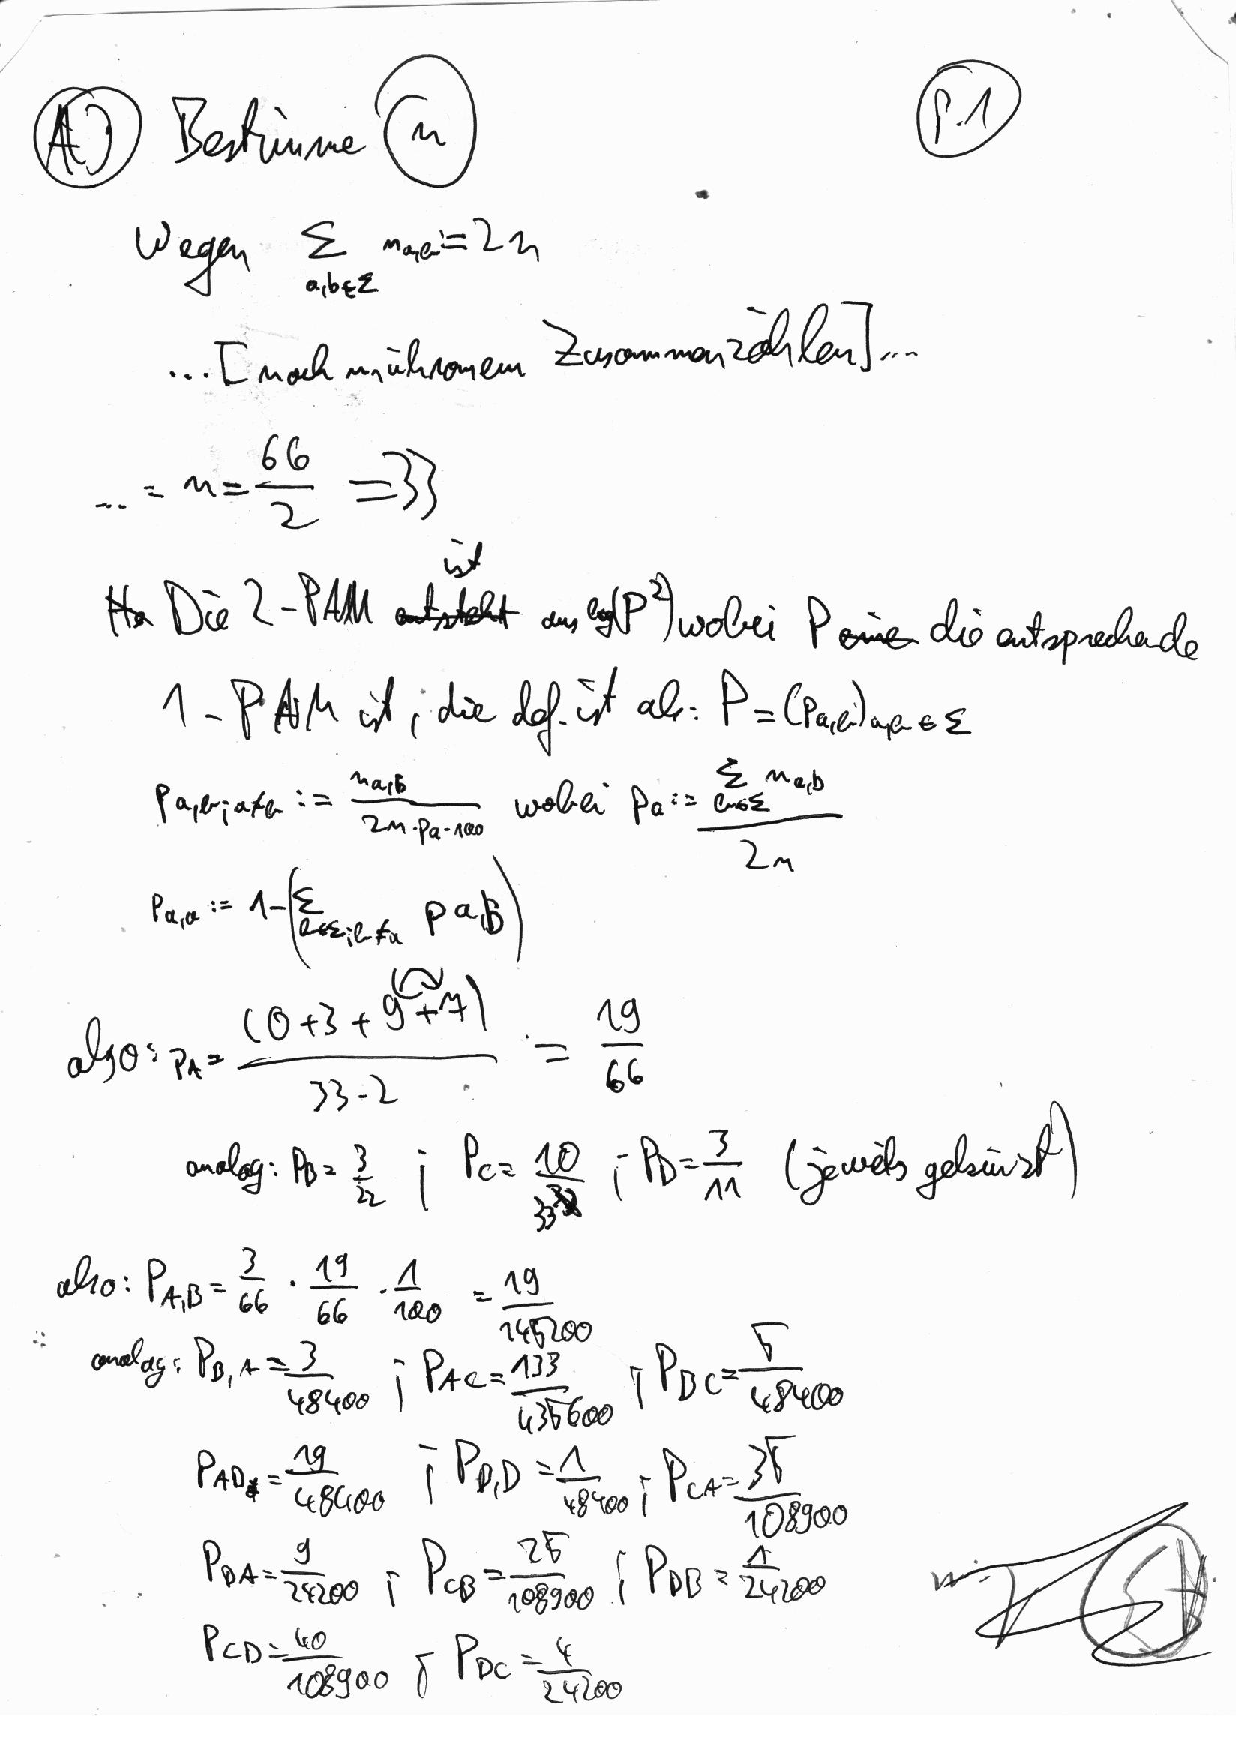
\includepdf[pages=-]{A3.pdf}

\end{document}
















